\documentclass{article}
\usepackage{my_style}
\usepackage{graphicx} % Required for inserting images
\usepackage{natbib}

\title{Review on CGK Embedding}
\author{}
\date{}

\begin{document}

\maketitle

\noindent 
The paper describes two methods: 

\begin{enumerate}
    \item [Embedding] This embeds the 2 strings $x$ and $y$ into $f(x,r)$ and 
    $f(y,r)$ using a random string $r$ which creates $3n$ hash functions 
    $h_1,h_2,...,h_{3n}: \{0,1\} \rightarrow \{0,1\}$.
    $\therefore f(x,r): \{0,1\}^n \times \{0,1\}^{6n} \rightarrow \{0,1\}^{3n}$.
    We compare and get the Hamming distance of $f(x,r)$ and $f(y,r)$ and claim
    that:
    $$\frac{1}{2}\cdot \Delta_e(x,y) \leq \Delta_H(f(x,r),f(y,r)) \leq
    O((\Delta_e(x,y))^2)$$
    with probability atleast 2/3.

    \item [Kernelization] This converts $x$ and $y$ into $x'$ and $y'$ such 
    that $\Delta_e(x,y)=\Delta_e(x',y')$. It uses the following 2 methods:
    \begin{enumerate}
        \item [Deflation] We increase the length of $x$ and $y$ and keep the 
        EditDistance same. We can prove that there exists a substring $w$ 
        in $x$ and $y$ of the form $w=p^r$ where $p$ is the periodicity of $w$
        and $r>2$. Somewhere in $w$, the strings $x$ and $y$ would align wrt
        EditDistance, as $w$ is same in both the strings $x$ and $y$, all the 
        bits after would be aligned too. We can add $p$ sometime after the initial 
        alignment index such that $w'=p^{r+1}$ and $\Delta_e(x,y)=\Delta_e(x',y')$

        \item [Shrinkage] Similar to the above case, we can remove $p$ bits form
        $w$ and the EditDistance would remain the same. In case of 
        \textbf{Shrinkage}, we define $s=K+2k+(k+1)(t+1)$ and reduce $w$ by
        keeping the first $s$ and last $s$ bits.
    \end{enumerate}
    Decompose $x=u_0w_1u_1...w_lu_l$ and $y=v_0w_1v_1...w_lv_l$, deflate and 
    shrink each $w_i$ to get the desired $x'$ and $y'$.
\end{enumerate}

\noindent
\textbf{Note:} this paper only compares 2 binary strings with low edit distance
$O(n^{1/6})$, where $n$ is the length of both the strings.

\pagebreak
\section*{Theorems and Proofs}
\begin{theorem}[\textbf{Theorem 4} in \cite{CGK16}] 
    The mapping $f:\{0,1\}^n \times \{0,1\}^{6n} \rightarrow \{0,1\}^{3n}$ 
    computed by Algorithm 1 satisfies the following condtions:
    \begin{enumerate}
        \item For every $x \in \{0,1\}^n$, given $f(x,r)$ and $r$, it is possible
        to decode back $x$ with probability $1-exp(-\Omega(n))$
        \item For every $x,y \in \{0,1\}^n$, $\Delta_e(x,y)/2 \leq \Delta_H(f(x,r),f(y,r))$
        with probability at least  $1-exp(-\Omega(n))$
        \item For every positive constant $c$ and every $x,y \in \{0,1\}^n$, 
        $\Delta_H(f(x,r),f(y,r))\leq c \cdot(\Delta_e(x,y))^2$ with probability
        at least $1-\frac{12}{\sqrt{c}}$
    \end{enumerate}
\end{theorem}

\begin{proof}[\textbf{Proof}]
    \begin{enumerate}
        \item we can decode back $x$ if we are given $f(x,r)$ and $r$ only if 
        the value of $i$ from Algorithm 1 is $n+1$ at the end of $f(x,r)$. As
        this would mean that we have traversed through all the bits of $x$.\\
        Consider that we have infinite hash functions 
        $h_1,h_2,...:\{0,1\}\rightarrow\{0,1\}$.\\
        Consider for each $x_i$ we embed it using hash functions $h_k,...,h_l$.
        As we embed $x_i$ for all $h_k,...,h_l$, it implies that 
        $h_k(x_i)=...=h_{l-1}(x_i)=0$ and $h_l(x_i)=1$.\\
        Hence, we can interpret the given condition as $n$ geometric distributions,
        where the total number of trials required is less than $3n$.\\
        \\
        For every grometric distribution, $p=1/2$.\\
        Define, $X_i = \text{Number of hash functions used to embed }x_i$, and
        all the $X_i$ are i.i.d\\
        \begin{align}
            E[X_i] &~=~ 2 \nonumber \\
            \therefore E[X] &~=~ 2n \nonumber        
        \end{align}
        Using Equation (6) from \cite{HR90}
        \begin{align}
            \Pr(S\geq(1+\epsilon)m) &~\leq ~e^{-\epsilon^2m/3} \nonumber\\
            (1+\epsilon)&~=~3/2 \nonumber\\
            \epsilon&~=~1/2 \nonumber\\
            \Pr(X>3n)&~\leq ~e^{-\frac{(1/2)^22n}{3}} \nonumber\\
            &~\leq ~e^{-n/6} \nonumber \\
            \therefore \Pr(X<3n) &~\geq ~1-e^{-n/6} \nonumber
        \end{align}
        
        \item $y$ differs from $x$ only in the parts where $f(x,r)\neq f(y,r)$.\\
        $f(x,r)_j\neq f(y,r)_j \Longrightarrow x_{i_x(j)}\neq y_{i_y(j)}$\\
        If $l=\Delta_H(f(x,r),f(y,r))$, then $x_{i_x(j)}\neq y_{i_y(j)}$ in atmost
        $l$ places.\\
        Define the following edit operations:\\
        \begin{align*}
            h_j(f(x,r)_j),h_j(f(y,r)_j) &~=~ (0,0) &&, \text{ignore} \nonumber\\
            &~=~ (0,1) &&,insert \nonumber \\
            &~=~ (1,0) &&,delete \nonumber \\
            &~=~ (1,1) &&,replace \nonumber
        \end{align*}
        We ignore at (0,0) as $(j+1)^{th}$ index would have the same values.\\
        Hence, the number of edit operations required would be less than or equal to the 
        hamming distance. \\
        Except, we need to consider the case where $0$s at the end of $x$ or $y$ 
        coincide with the trailing $0$s, in this case, the actual bit flips required
        would be $2l$.\\
        Hence, $\Delta_e(x,y) \leq 2*\Delta_H(f(x,r),f(y,r))$.\\


        \item This can be proved by combining \textbf{Lemma 4.2} and 
        \textbf{Proposition 3.2}.\\
        \textbf{Lemma 4.2}: 
        \begin{align}
            \Pr(\Delta_H(f(x,r),f(y,r))\leq l) &~\geq~ 
            \sum_{t=0}^{l} q(t,\Delta_e(x,y))\nonumber\\
            \text{For our case, $l=c\cdot (\Delta_e(x,y))^2$} \nonumber\\
            \Pr(\Delta_H(f(x,r),f(y,r))\leq c\cdot (\Delta_e(x,y))^2) &~\geq~ 
            \sum_{t=0}^{c\cdot (\Delta_e(x,y))^2} q(t,\Delta_e(x,y)) \nonumber\\
            \text{From \textbf{Proposition 3.2},} 
            \sum_{t=0}^{l} q(t,k) \geq 1- \frac{12k}{\sqrt{l}} \nonumber \\
            \Pr(\Delta_H(f(x,r),f(y,r))\leq c\cdot (\Delta_e(x,y))^2) &~\geq~ 
            1-\frac{12\Delta_e(x,y)}{\sqrt{c\cdot (\Delta_e(x,y))^2}}  \nonumber \\
            &~\geq~ 1-\frac{12}{\sqrt{c}} \nonumber
        \end{align}
    \end{enumerate}
\end{proof}

\begin{lem}[\textbf{Lemma 4.2} in \cite{CGK16}] 
    Let $x,y \in \{0,1\}^n$ be of edit distance $\Delta_e(x,y) = k$. Let $q(t,k)$
    be the probability that a random walk on the integer line starting from the 
    origin visits the point $k$ at time $t$ for the first time. Then for any
    $l>0$, $\Pr(\Delta_H(f(x,r),f(x,y)) \leq l) \geq \sum_{t=0}^{l} q(t,k)$ 
    where the probability is over the choice of $r$.
\end{lem}

\begin{proof}[\textbf{Proof}]
    \textit{Example:}\\
    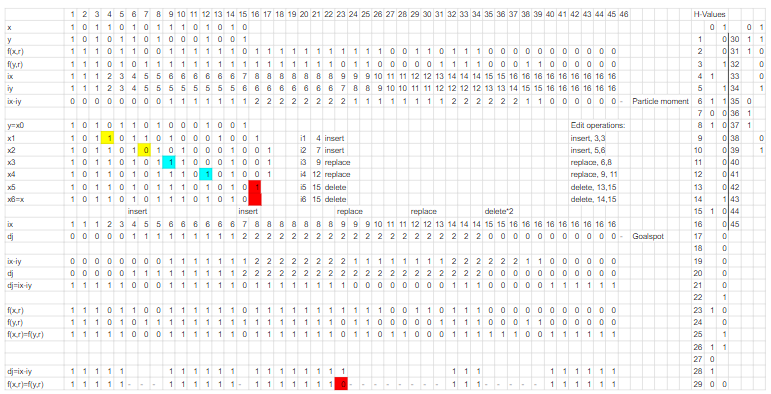
\includegraphics{./utils/CGK_Lemma4.2.png}\\
    \begin{enumerate}
        \item In the above image, we have the value of $x$, $y$, $f(x,r)$ and 
        $f(y,r)$ (based on the H-values mentioned on the right side).\\
        The values $i_x$ and $i_y$ are the indices of $x$ and $y$ for the given 
        $f$ values.\\

        \item \textbf{Particle Moment:}
        Every step taken by the particle is defined as $h_j(x_{i_x(j)})-h_j(y_{i_y(j)})$,
        for $j^{th}$ value of $f(x,r)$ and $f(y,r)$.\\
        Now, $\sum_{k=0}^{j} h_j(x_{i_x(k)}) = i_x(j)-1$ and 
        $\sum_{k=0}^{j} h_j(y_{i_y(k)}) = i_y(j)-1$, as the $i$ value changes
        only when $h()=1$. \\
        Hence, $h_j(x_{i_x(j)})-h_j(y_{i_y(j)})=i_x(j)-i_y(j)$.\\
        Hence, the position of particle at time $j$ is $i_x(j)-i_y(j)$.

        \item \textbf{Goalspot:}
        We define $y=x^{(0)},x^{(1)},...,x^{(k)}=x$ as a series of $k$ strings
        such that the first string is $y$ and the last string is $x$ and 
        $\Delta_e(x^{(l-1)},x^{(l)})=1$.\\
        $\therefore$, in the above image, each $x^{(l)}$ is mentioned. The
        inserted bits are colored yellow, replaced bits are colored blue and 
        deleted bits are colored red. The edit operation from $x^{(1)},x^{(6)}$
        are: insert, insert, replace, replace, delete, delete. The first index $(i^{(l)})$
        where $x^{(l)}$ differs from $x^{(l-1)}$ is 4, 7, 9, 12, 15, 15 respectively.\\
        We define $d_j$(goalspot) as:\\
        $d_0=0$ \\
        when $i_x(j)=i^{(l)}$ for the first time, if the corresponding edit
        operation is:\\
        \begin{align}
            \text{insert } &\Longrightarrow \text{ increment } d_j \text{ by 1} \nonumber\\ 
            delete &\Longrightarrow \text{ decrement } d_j \text{ by 1 } \nonumber\\
            otherwise &\Longrightarrow \text{ do not change } d_j \nonumber
        \end{align}
        \\
        \item Idle state:
        \begin{equation}
        \label{idle}
         d_j=i_x(j)-i_y(j) \Longrightarrow x_{i_x(j)}=y_{i_y(j)}    
        \end{equation}
        When $d_j=i_x(j)-i_y(j)$, the $x$ and $y$ strings are aligned at 
        that point $\Longrightarrow x_{i_x(j)}=y_{i_y(j)} \Longrightarrow f(x,r)_j=f(y,r)_j$\\
        $x$ and $y$ would continue to be in alignment (defined as the idle state)
        unless and until $d_j$ does not change, i.e. we do not 
        encounter an edit operation.\\

        \item We can verify from the above image, when $d_j=x_{i_x(j)}-y_{i_y(j)}$
        then $f(x,r)_j=f(y,r)_j$.\\
        \textit{Except,} when we have replace operation (the cell marked red in 
        the last row). Because in case of replace, $x$ and $y$ are aligned, but
        their values are different. Ergo, the system won't be in an idle state.

    \end{enumerate}

    \textbf{Kennel Struggle:} \\
    
    \begin{enumerate}
        \item \textbf{Kennel} $\equiv$ Goalspot.
        \item \textbf{Cat} $\equiv$ Particle. Cat has a random moment \{-1,0,+1\}
        with probability \{1/4,1/2,1/4\}.
        \item \textbf{Dog} $\equiv$ Edit distance. The dog is incharge of moving 
        the kennel. The actions involve moving the kennel to the left($\equiv$ 
        Deletion), moving the kennel to the right($\equiv$ Insertion), barking
        ($\equiv$ Bit flip). The Dog disappears after $k$ steps. 
        \textbf{Note:} When the Cat reaches the Kennel, the dog has to make a 
        move because Cat reaching the Kennel $equiv$ Particle=Goalspot, referring
        to \ref{idle}, this would mean that the system is in idle state and would
        continue to remain in idle state unless the value of $d_j$ does not 
        change.
    \end{enumerate}
    \textbf{Success Scenario:} Cat reaches an empty Kennel.\\
    Probability of Cat reaching an empty Kennel in $l$ steps is least if the dog
    uses the following strategy:\\
    \begin{enumerate}
        \item Move the Kennel to the left by 1 position
        \item Wait until the cat reaches the Kennel
        \item Move the Kennel to left by 1 position
    \end{enumerate}
    As Dog has $k$ 
    moves, the above process will repeat $k$ times.\\
    \\
    The probability that the Cat reaches position 1 for the first time in t moves is given by
    $q(t,1)$. Hence for $k$ steps, we have 
    $\sum_{t_1+t_2+...+t_k<l}^{}(q(t_1,1)q(t_2,1)...q(t_k,1))$.\\
    Hence,
    \begin{align}
        \Pr(\text{Cat reaches empty Kennel in atmost}l\text{ steps}) & ~\geq ~\sum_{t_1+t_2+...+t_k\leq l}^{}(q(t_1,1)q(t_2,1)...q(t_k,1)) \nonumber \\
        \Pr(\text{Cat reaches empty Kennel in atmost}l\text{ steps}) & ~\geq ~
        \sum_{t\leq l}^{}q(t,k) \nonumber \\
        \mathclap{\text{As the Particle moment is defined by }h_j(x_{i_x(j)})-h_j(y_{i_y(j)})
        \text{, the Particle would move only when }x_{i_x(j)}\neq y_{i_y(j)}} \nonumber\\
        \Pr(\Delta_H(f(x,r),f(y,r))\leq l) & ~\geq ~
        \sum_{t\leq l}^{}q(t,k) \nonumber \\
        \Pr(\Delta_H(f(x,r),f(y,r))\leq l) & ~\geq ~
        \sum_{t=0}^{l}q(t,k) \nonumber 
    \end{align}
\end{proof}


\bibliographystyle{alpha}
\bibliography{refs}

\end{document}
